The goal of indexing is to improve the efficiency of searches. For spatial indexing, the goal is to improve the efficiency of processing spatial queries. Spatial queries relate to the attributes of spatial objects such as their positions and sizes and whether or not they intersect with each other. This can be achieved with spatial data structures such as the R-tree.

\section{Concepts}

A spatial object can be a point, a line, a polygon, or any other shape in the real coordinate space of \(d\) dimensions \(\mathbb{R}^d\). Using set theory, a spatial object in \(\mathbb{R}^d\) can be considered a potentially infinite set of points \(X\) such that \(X \subseteq \mathbb{R}^d\).

Set operations have geometric interpretations. As an example, given two spatial objects \(X\) and \(Y\), \(X \cap Y\) is a spatial object consisting of the space covered by both objects, which is the intersection of the two objects.

A spatial predicate is a relation between spatial objects. For instance, given spatial objects \(U\) and \(V\), \(U\) and \(V\) are said to intersect if \(U \cap V \neq \emptyset\), and \(U\) is said to contain \(V\) if \(U \supseteq V\). Spatial predicates may have properties that are useful for processing spatial queries. For instance, any object that contains an object \(U\) that intersects with an object \(V\) must also intersect with \(V\).

A point \(p\) in \(d\)-dimensional space can be represented as a \(d\)-dimensional vector \((p^{[1]}, p^{[2]}, \dotsc, p^{[d]})\) where \(p^{[i]}\) denotes the \(i^{th}\) coordinate of \(p\). A point may be a spatial object in the form of a singleton, which is a set with exactly one element, the point itself.

An axis aligned box is a spatial object in the form of a box where the edges of the box are parallel to the coordinate axes. An axis aligned box is defined by two points \(B = (b, t)\) where
\[
  \forall i \in \{1, \dotsc, d\} :
  b^{[i]} \leq t^{[i]}
\]
where \(p^{[i]}\) denotes the \(i^{th}\) coordinate of the point \(p\). \(b\) can be considered the \emph{bottom point} and \(t\) can be considered the \emph{top point}. The axis aligned box contains points so that for each dimension \(i\), \(b^{[i]}\) is the minimum (bottom) coordinate and \(t^{[i]}\) is the maximum (top) coordinate. That is,
\[
  B = \{
    q \in \mathbb{R}^d \mid
    \forall i \in \{ 1, \dotsc, d \} :
    b^{[i]} \leq q^{[i]} \leq t^{[i]}
  \}
\]

The axis aligned Minimum Bounding Box (MBB) of a spatial object \(X\) is the axis aligned box with the smallest measure that covers \(X\). Depending on the dimensionality of the space, the measure of a spatial object can be the length, area, volume or hypervolume of the object. Axis aligned MBBs are commonly used to approximate the locations of spatial objects and can be used as a simple descriptor of the shape of a more complex spatial object.

It follows that that \(X \subseteq \textrm{MBB}(X)\), which implies that any spatial object that intersects with \(X\) must also intersect with \(\textrm{MBB}(X)\). For complex geometry, this has practical applications to speed up computations for spatial operations.

The axis aligned MBB of a spatial object \(X\) can be represented as \(B = (b, t)\) where
\[
  \forall i \in \{ 1, \dotsc, d \} :
  b^{[i]} = \min\left( q^{[i]} \mid q \in X \right)
  ,
  t^{[i]} = \max\left( q^{[i]} \mid q \in X \right).
\]

\section{Spatial join queries}

The spatial distance join returns pairs of objects that are close to each other. More formally, given two sets of spatial objects \(R\) and \(S\), a distance metric dist and a distance threshold \(\epsilon\), the spatial distance join returns
\[
  \{ (r, s) \in R \times S \mid \mathrm{dist}(r, s) \leq \epsilon \}.
\]

\(dist\) is defined to return the distance between the points of the two spatial objects that are closest to each other according to a distance function \(p\).

\[
  dist(r, s) = \min\left(p(t, u) \mid t, u \in r \times s \right)
\]

For instance, \(p\) could be the Euclidean distance, which is the straight-line distance between two vectors. We can also use the Chebyshev distance, where the distance is the greatest of the differences along any coordinate dimension.

\(dist(r, s) \leq \epsilon\) is a type of spatial predicate. For \(\epsilon = 0\) it is equivalent to intersection. Using the Chebyshev distance measure between two bounding boxes \(r\) and \(s\), we can think of it as expanding either \(r\) or \(s\) by \(\epsilon\) and testing for intersection.

For the purposes of spatial indexing, the distance metric will primarily operate on points and axis aligned boxes. This simplifies finding the pair of points that are closest to each other according to the distance function. For pairs of spatial objects that are points, the distance function is simply computed directly on the points. For pairs of spatial objects that are axis aligned boxes, the closest points can be found on the box boundaries, unless the boxes intersect, in which case the distance is zero.

\section{R-trees}

The R-tree~\cite{guttman1984r} can be considered a multidimensional version of the B-tree, which is a balanced search tree. The keys of the R-tree are axis aligned boxes which can be spatially queried. It is commonly used as an indexing structure for spatial queries.

Conceptually, the R-tree partitions the key space into a hierarchy of MBBs where key boxes are placed at the bottom. Each MBB in the hierarchy consists of the MBB of its children. MBBs at the same level in the hierarchy may overlap with each other.

The R-tree is a balanced tree structure consisting of a number of nodes divided into levels. Nodes in all levels but the lowest level are inner nodes, while nodes at the lowest level are leaf nodes. Entries are placed in the leaf nodes, each containing a link to a data object along with the key box. Inner nodes contain similar entries, except they link to lower level nodes instead of data objects along with the MBB of the lower level node. A leaf node is said to contain a data object if any of its entries point to the data object. Similarly, an inner node is said to contain a data object if any of its ancestor leaf nodes contain the data object. In figure \ref{fig:r-tree}, A is the root node, which is an inner node. B, C and D are leaf nodes which are entries of the root node. E, F, G, H, I and J are leaf node entries.

\begin{figure}[h]
    \centering
    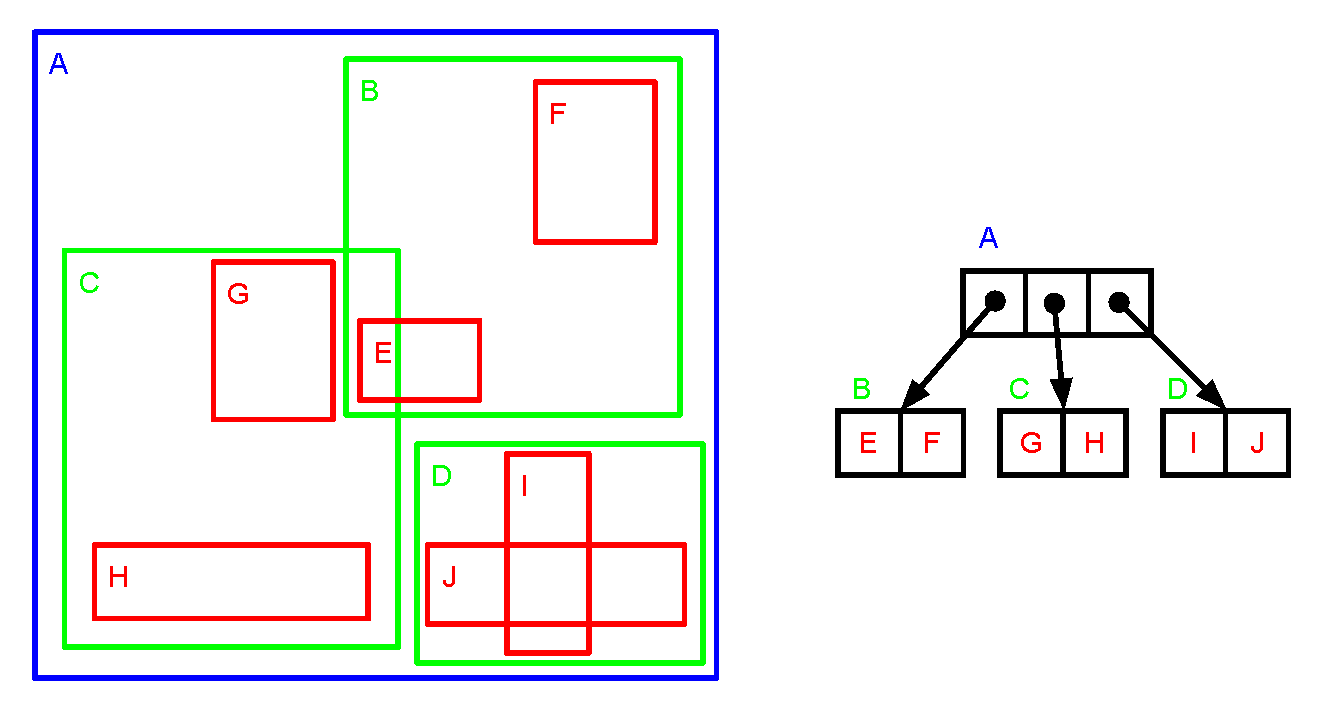
\includegraphics[scale=0.5]{r_tree}
    \caption{R-tree}
    \label{fig:r-tree}
\end{figure}

Values are inserted as entries in leaf nodes. To keep the tree balanced and to avoid nodes growing too large, all nodes but the root node must have between \(m\) and \(r\) entries where \(m \leq \frac{r}{2}\). \(r\) is the maximum amount of entries in an R-tree node, and is called the \emph{fanout}. The root node can have anywhere from \(0\) to \(r\) entries. If inserting an entry into a leaf node would result in more than \(r\) entries, the node has to be split into two leaf nodes by creating a new leaf node and partitioning the entries between them. The newly created leaf node has to be inserted into the parent node, which may result in the parent node requiring a similar split. The split can propagate up to the root, in which case the root also must be split, and another level has to be added to the tree.

The query performance of an R-tree is a measure of the average amount of nodes that have to be visited to perform a search. When searching, it is desirable to visit as few nodes as possible, as each branch of each node has to be evaluated, and accessing a node may have a cost (depending on the memory layout). For good query performance, R-tree nodes should be packed as fully as possible, and branches should have minimal overlap. Packed nodes decrease the height of the tree, which reduces the amount of nodes that have to be accessed to reach the leaves. When the cost of accessing a node outweighs the cost of evaluating branches, packed nodes reduce the total amount of nodes which results in fewer nodes that have to be accessed to perform a search. Minimal overlap between branches allows the search to more easily narrow down to fewer subtrees.

The R-tree has been extensively researched and used, and has inspired the creation of variations such as the R*-tree~\cite{beckmann1990r}, the R+-tree and the revised R-tree. Most of the variations preserve the data structure and principles while redefining the insert and remove operations. Operations that modify the tree can be designed for varying degrees of query performance at the cost of the performance and complexity of operations to insert and delete values.

\subsection{aR-trees}

The aR-tree is an R-tree that has been augmented with aggregate values assigned to each node. Similar to how the MBB of a node is an aggregation of the boxes of all objects placed under it, other types of object attributes can be aggregated to enhance the search capabilities of the tree. An example aR-tree is the IR-tree~\cite{li2010ir} which is augmented for spatio-textual searches by storing aggregated inverted files in each node. A simpler example is an aR-tree that stores the maximum and minimum value of an attribute for all objects under the node, which may have practical applications in databases.

The aggregated attribute of an aR-tree node \(N.agg\) is defined by a value function \(v\) and a decomposable aggregate function \(\gamma\). \(v\) retrieves values from object that can be aggregated by \(\gamma\). For leaf nodes, the aggregate value is computed directly as the aggregation of \(v\) for all objects contained by the leaf node. For inner nodes, the aggregate value is computed as the aggregation of the \(N.agg\) values of its child nodes. It follows that the aggregate value of any node is the aggregation of \(v\) for all R-tree entries under the node.

The aggregate values stored in the aR-tree augment the search capabilities of the R-tree because each inner node carries information that can be used to assert certain properties about contained values. By using the MAX aggregate function on \(v(O)\) when searching for objects with the condition \(v(O) \geq v_{\min}\), it can be asserted that only inner nodes with \(N.agg \geq v_{\min}\) can contain values satisfying the condition. The MAX aggregate function also guarantees that the entry with the greatest \(v(O)\) can be found by descending the tree and always choosing the inner node with the greatest aggregate value.

\begin{figure}[h]
    \centering
    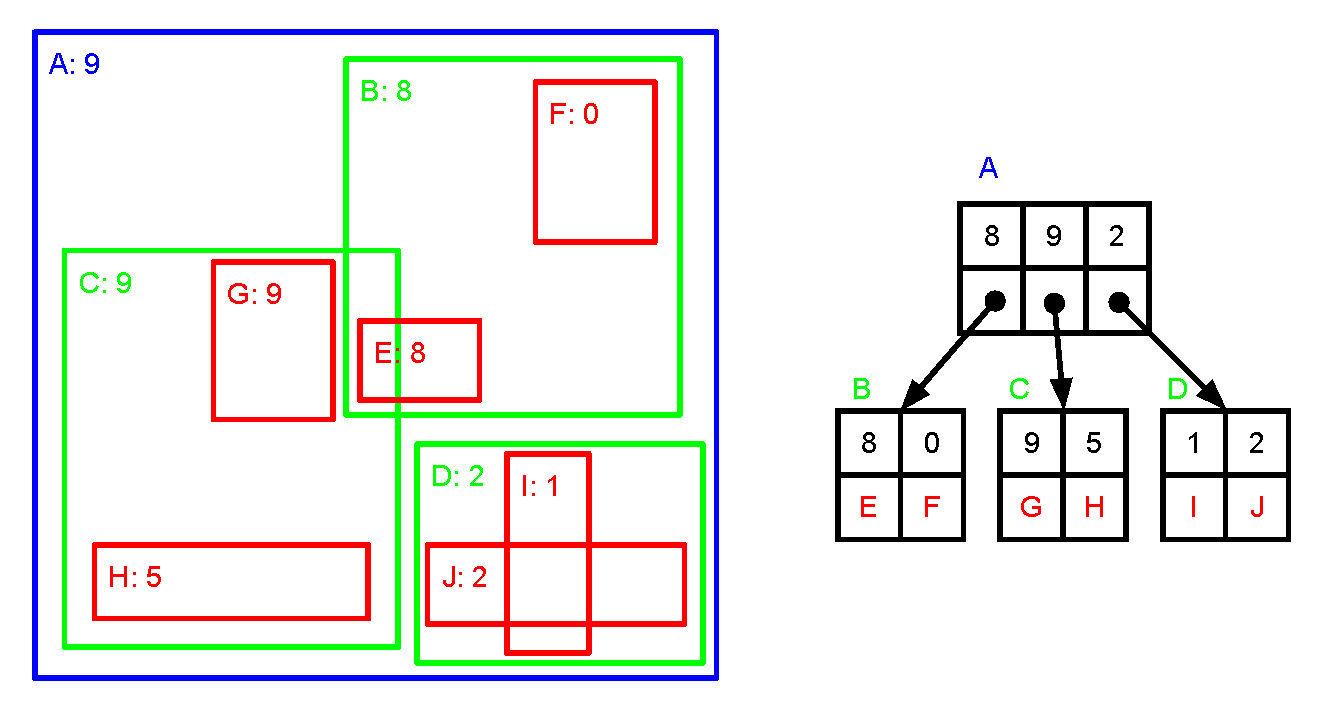
\includegraphics[scale=0.5]{max_ar_tree}
    \caption{MAX aR-tree}
    \label{fig:max-ar-tree}
\end{figure}

% Operations that modify aR-trees require updating the aggregate values. When an entry with aggregate value \(s\) is added to a node \(N\), either as \(s = v(O)\) for an object \(O\) or as \(s = M.agg\) for a node \(M\), the aggregate value of \(N\) can be updated as \(N.agg' = \gamma(N.agg, s)\). When an entry is removed from a node, the aggregate value of the node has to be recomputed from the remaining entries.

\subsection{Range search using R-trees}

A range search on an R-tree returns the leaf entries whose MBBs intersect with the query box. Algorithm~\ref{alg/r-tree-range-search} can be described as an iterative operation on a LIFO (Last-In-First-Out) queue. The queue is initialized with the entries of the root node. Entries are dequeued until the queue is empty. If the dequeued entry is a leaf node entry, it is made part of the result. If the entry is an inner node entry, all its children are enqueued. A query box that does not intersect with the MBB of a node \(N\) cannot intersect with any objects contained by \(N\). Therefore, a non-intersecting node and all its ancestors can be pruned from the search because they will not output any results.

\begin{algorithm}
  \caption{R-tree Range Search. \(N\) is any R-tree node, but usually the root node of the R-tree. \(Q\) is the query box.}
  \label{alg/r-tree-range-search}
  \begin{algorithmic}[1]
    \Function{RangeSearch}{\protect\(N, Q\protect\)}
      \State \(O \leftarrow \emptyset\)
      \State Initialize \(Queue\) as a queue with entries of \(N\).
      \While{\(Queue\) is not empty}
        \State \(E \leftarrow\) \Call{Dequeue}{\protect\(Queue\protect\)}
        \If{\Call{Intersects}{\protect\(E.mbb, Q\protect\)}}
          \If{\(E\) is a leaf entry}
            \State \(O \leftarrow O + E\)
          \Else
            \ForAll{\(C \in E.ref\)}
              \State \Call{Enqueue}{\protect\(Queue, C\protect\)}
            \EndFor
          \EndIf
        \EndIf
      \EndWhile
      \State \Return \(O\)
    \EndFunction
  \end{algorithmic}
\end{algorithm}

While range search concerns spatial intersection with a query box, it is possible to generalize for other predicates provided they have a similar property. The specific property required of a predicate \(\phi\) is as follows,
\[
  \forall A, A' \in \mathbb{P}(\mathbb{R}^d) : (A \subseteq A') \wedge \phi(A) \Rightarrow \phi(A')
\]
where \(\mathbb{P}(\mathbb{R}^d)\) is the set of all spatial objects in the \(d\)-dimensional space \(\mathbb{R}^d\). An interpretation is that a if the predicate is true for a spatial object \(A\), it must also be true for any larger object that contains \(A\). In the case of an R-tree range query, \(\phi\) tests for intersection with a query box, where \(A\) is a box of a leaf node entry and \(A'\) is the MBB of any node that contains it. If an entry in an R-tree intersects with the query box, any node that contains the entry must also intersect with the query box, otherwise it would be pruned during the range search.

\subsection{Spatial join using R-trees}

R-trees can naturally be used to enhance the performance of spatial joins. As opposed to performing a nested loop join to test the spatial predicate for all pairs, R-trees can utilize the spatial characteristics of the inputs to reduce the amount of spatial predicate evaluations necessary to produce the output. R-trees can be built dynamically similarly to hash tables for relational joins, or they can be joined directly.

Brinkhoff et al.~\cite{brinkhoff1993efficient} described a method to concurrently descend down two R-trees to perform a spatial intersection join as described in algorithm \ref{alg-r-tree-spatial-intersection-join}. The algorithm is quite similar to the range search algorithm, except it searches for leaf entry tuples instead of individual leaf entries. Similar to the pruning in the range search algorithm, the spatial intersection join is based on the idea that if the MBBs of nodes \(N_R\) and \(N_S\) do not intersect, the objects they contain cannot form pairs \((key_R, key_S)\) where \(key_R\) and \(key_S\) intersect. Given well constructed R-trees, this allows pruning potential intersecting candidates at directory levels.

\begin{algorithm}
  \caption{R-tree Spatial Intersection Join. \(N_R\) and \(N_S\) are R-tree nodes from R-trees \(R\) and \(S\), usually the root nodes of their respective R-trees.}
  \label{alg-r-tree-spatial-intersection-join}
  \begin{algorithmic}[1]
    \Function{SpatialJoin}{\protect\(N_R,N_S\protect\)}
      \Comment{\(N_R\) and \(N_s\) must be at the same level}
      \State \(O \leftarrow \emptyset\)
      \State Initialize \(Queue\) as a queue with entry pairs of \(N_R \times N_S\).
      \While{\(Queue\) is not empty}
        \State \((E_R, E_S) \leftarrow\) \Call{Dequeue}{\protect\(Queue\protect\)}
        \If{\Call{Intersects}{\protect\(E_R.mbb, E_S.mbb\protect\)}}
          \If{\(E\) is a leaf entry}
            \Comment{\(S\) is also a leaf}
            \State \(O \leftarrow O + (E_R, E_S)\)
          \Else
            \ForAll{\(C_R \in E_R.ref\)}
              \ForAll{\(C_S \in E_S.ref\)}
                \State \Call{Enqueue}{\protect\(Queue, (C_R, C_S)\protect\)}
              \EndFor
            \EndFor
          \EndIf
        \EndIf
      \EndWhile
      \State \Return \(O\)
    \EndFunction
  \end{algorithmic}
\end{algorithm}

Like the range query, the algorithm can be described as an iterative operation on a LIFO (Last-In-First-Out) queue. The queue is initialized with all root node entry combinations. Tuples of branches are dequeued until the queue is empty. If the dequeued entries are leaf node entries, they are made part of the result. If the entries are inner node entries, all combinations of children entries are enqueued. A pair of nodes that do not intersect cannot contain intersecting entries. Therefore, tuples of non-intersecting nodes and all their ancestor tuples can be pruned from the search because they will not output any results.

For R-trees with different height, a more complete solution is required. In the case where \(S\) is taller than \(R\), the SpatialJoin algorithm will output entries \((E_R, E_S)\) where \(E_R\) is a leaf node entry in \(R\) while \(E_S\) is an inner node entry in \(S\) instead. In order to produce the expected spatial join outputs, for each output of SpatialJoin, a range search must be performed on the node referenced by \(E_S\) using \(E_R\mathrm{.mbb}\) as the query box. The output of the range search on \(E_S\) can then be output as tuples with \(E_R\).

While Brinkhoff et al.\@ only considered spatial intersection, it is possible to generalize for other spatial predicates provided they have a similar property. The specific property required of a spatial predicate \(\phi\) is as follows,
\[
  \forall A, A', B, B' \in \mathbb{P}(\mathbb{R}^d) : (A \subseteq A') \wedge (B \subseteq B') \wedge \phi(A, B) \Rightarrow \phi(A', B')
\]
where \(\mathbb{P}(\mathbb{R}^d)\) is the set of all spatial objects in the \(d\)-dimensional space \(\mathbb{R}^d\). An interpretation is that if the predicate is true for a pair of spatial objects \(A\) and \(B\), it must also be true for any pair of larger objects that contain \(A\) and \(B\). In the case of an R-tree join, \(A\) and \(B\) are boxes of leaf node entries from their respective R-trees, and \(A'\) and \(B'\) are the MBBs of nodes containing them. If entries of two R-trees intersect with each other, any node that contains the entries from each tree must also intersect with each other, otherwise they would be pruned during the range search.

The generalization of spatial predicates for range search and spatial joins is a necessary insight to apply the algorithms for other predicates than intersection. The property is intuitively true for the intersection predicate. The spatial distance threshold predicate can be considered equivalent to intersection where either object is \emph{expanded} by \(\epsilon\), therefore the property intuitively holds true for the spatial distance predicate.

\subsection{Search types and iterators}

Queues can be implemented in various ways for range searches with R-trees to create different kinds of searches. By replacing the LIFO queue with a FIFO queue, the search becomes a breadth-first search (BFS) instead of a depth-first search (DFS). When the order of the output matters, the queue can also be replaced by a priority queue to perform a best-first search, which has applications for ranked queries. aR-trees can provide necessary attributes to sort entries of inner nodes in the priority queue. Because the R-tree join is also based on a queue, similar results can be achieved.

A depth-first-search can be performed using a compact tree search iterator such as the one described in algorithm~\ref{alg-tree-search-iterator} instead of using an explicit queue. The iterator operates on a stack of node entry iterators. The stack will contain at most an iterator per level of the R-tree, and therefore has a fixed capacity equal to the height of the R-tree. The node entry iterator may simply be based on a pointer to an R-tree node and a number that counts the number of entries of the node that have been visited. The tree search iterator can also be applied to spatial joins by replacing the node entry iterator with an iterator that joins the entries of two nodes.

\begin{algorithm}
  \caption{DFS Tree Search Iterator. \(S\) is a stack of node entry iterators, initialized with a node entry iterator of the root node. \(\phi\) is the search predicate used to prune R-tree entries.}
  \label{alg-tree-search-iterator}
  \begin{algorithmic}[1]
    \Function{Next}{\protect\(S, \phi\protect\)}
      \While{\(S\) is not empty}
        \State \(I \leftarrow\) \Call{Peek}{\protect\(S\protect\)}
        \State \(E \leftarrow\) \Call{Next}{\protect\(I, \phi\protect\)}
        \If{\(E\) is Nil}
          \State \Call{Pop}{\protect\(S\protect\)}
        \Else
          \If{\(E\) is inner node entry}
            \State \(I_C \leftarrow\) \Call{NodeEntryIterator}{\protect\(E\protect\)}
            \State \Call{Push}{\protect\(S, I_C\protect\)}
          \Else
            \State \Return \(E\)
          \EndIf
        \EndIf
      \EndWhile
      \State \Return Nil
    \EndFunction
  \end{algorithmic}
\end{algorithm}

An explicit queue based search allows for parallel processing of queue elements by having multiple threads dequeuing and enqueuing elements in the same queue. This method can achieve data parallelism by both evaluating spatial predicates and traversing subtrees in parallel, but requires efficient synchronization mechanisms for the queue. The efficiency of this method depends on the amount of elements that can be processed in parallel, which may be limited by the amount of queue elements produced at each level in the search. For a narrow range search in a well constructed R-tree, the number of subtrees that must be visited should be low, which results in an overall small queue until the last few levels. Therefore, the gains for range queries would primarily be in parallel evaluation of spatial predicates. However, the queue is expected to grow exponentially for an R-tree spatial join, which suggests that parallel evaluation of spatial joins can be limited by the amount threads available rather than the size of the queue.

One way to utilize parallel processing of queue elements in range search is processing multiple range queries in parallel using the same queue. You et al.~\cite{you2013parallel} proposed and evaluated multiple methods to perform parallel range queries using GPUs.\@ Given an R-tree and a set of range queries to be performed on the R-tree, the algorithms efficiently computes the result of all range queries in parallel. It can be done by implementing existing methods for depth-first and breadth-first search for R-tree range queries on the GPU.\@

In the DFS method, each thread processes one query in depth-first order using a DFS tree search iterator. The main advantage of DFS is its predictable memory usage and simplicity. Each query requires only a stack with capacity equal to the height of the tree to perform the traversal, which can be stored in shared memory. The implementation is based on a count-and-write strategy that spaces out the memory prior to writing the query results. An issue with the DFS method is that it provides poor workload balance when queries require different amounts of work, leaving some threads idle and waiting for others to finish. The count-and-write strategy effectively requires evaluating all queries twice, which is speculated to harm performance. For particularly large queries, the writing of results to global memory may also be too sparse to coalesce.

The BFS method distributes the queries across multiple thread groups where each thread group has a queue in shared memory and all its threads working on the queue in parallel. Each queue entry is a \((N, Q)\) tuple where \(N\) is a pointer to an R-tree node and \(Q\) identifies a query. A queue entry \((N, Q)\) is expanded by dequeuing then enqueueing the children of N as \((N_C, Q)\) tuples, but only if the MBB of \(N\) and the query box of \(Q\) intersect. When a queue contains only leaf nodes, it is copied to global GPU memory to be made part of the result. Compared to the DFS method, the BFS method solves the workload balance problem within each thread group and has superior performance overall, but is more complex due to the limited capacity of the queue.

As previously stated, each queue in the BFS method has a fixed capacity imposed by the limited amount of shared memory that is available to each thread group. In a breadth-first search, the queue is expected to grow larger as the search goes deeper and may cause the queue to overflow. Calculating a distribution of queries that avoids overflow is infeasible, therefore the algorithm is designed to handle overflows. There are multiple alternatives for overflow handling strategies, and the most promising alternative dynamically allocates chunks of global memory for overflowing queues.

Performing a set of range queries on an R-tree is equivalent to performing an R-tree join using an R-tree constructed from the set of range queries. Given that range queries can be performed in parallel using the DFS and BFS methods, spatial joins could also be performed in parallel by modeling the problem as a set of range queries on an R-tree, but it would lack the main strength of the R-tree join algorithm, which is its ability to prune subtrees of both R-trees.

Given the queue-based search nature of DFS, BFS and the R-tree spatial join algorithm, it may be possible to adapt the DFS and BFS methods to perform parallel spatial joins, but some differences must be tackled. By considering each element of the queue as an independent task that either produces subtasks or outputs values, execution of parallel range queries starts with a large queue and therefore a large set of independent tasks that can easily be distributed in DFS and BFS. A spatial join, however, starts with a single queue entry and therefore only a single task. To efficiently perform a spatial join as independent tasks, the initial task must first be broken down into independent tasks.

\subsection{Memory layout}

Being originally designed for disk storage, the original R-tree uses a page-based layout. Nodes correspond to disk pages if the structure is disk resident, and memory pages otherwise. An R-tree node with this layout can contain as many entries as the page can fit as records. A notable feature is that the MBB of an R-tree node is stored along with the pointer to the node's page in an inner node record instead of being stored within the node's own page. This allows pruning the node without having to load the page. Loading a disk resident page has a significant I/O cost, but a memory resident page may also have an access cost because the page may have to be loaded into processor cache. The main advantage of the page-based layout is that modifying the structure of the R-tree only requires allocating and freeing pages and updating pointers to pages.

A page based layout would be inefficient on GPU. One difficulty with using the page-based layout on GPUs is transferring R-trees between main memory and device memory. Every source page would have to be replicated in the other memory by allocating a destination page and performing a memory transfer between the source and the destination per page. Destination pages may receive different memory addresses in the destination memory, requiring pointers to be updated. Additionally, R-trees with read-only usage would not benefit from strength of the page-based layout, which is its performance for operations that modify the structure of the R-tree.

Luo et al.~\cite{luo2012parallel} used two arrays to store the R-tree structure on a GPU.\@ The first is an array of integers representing the tree structure which is called \emph{Index}, and the second is an array of boxes called \emph{Rect}. For an R-tree with \(N\) nodes and a fanout of \(r\), both arrays consist of \(N\) blocks of \(r\) values. The root node is stored in the first block of both arrays. For inner nodes, each integer in a block of \emph{Index} is the array index of a child node, and each box in a block of \emph{Rect} is the MBB of the child node. For leaf nodes, each integer in a block of \emph{Index} is an identifier of an entry in the R-tree, and each box in a block of \emph{Rect} is the box of the entry. Non-full nodes are padded by zeroes in \emph{Index}.

The linearized R-tree memory layout used by You et al.~\cite{you2013parallel} stores the entire R-tree in an array of all nodes in breadth-first order. Inner nodes are represented by \(\{MBB, pos, len\}\) tuples, where \(MBB\) is the minimum bounding box of the node, \(pos\) is the position of the first child node in the array, and \(len\) is the amount of children. Because sibling nodes are stored sequentially in BFS order, their positions can be calculated by offsetting from the position of the first child. The specific layout of leaf nodes was left unspecified. The linearized R-tree memory layout is more compact than the layout used by Luo et al.~because inner nodes do not store a position per child, and there is no wasted memory for nodes that are not filled to capacity.

The linearized R-tree memory layout is optimized for read operations and memory transfers without serialization. It is designed to be cache friendly with its compact layout and sequential sibling node storage. The entire R-tree can easily be streamed between main memory and GPU memory by only streaming the the array. It should only be used for read-only R-trees. Write operations would require shifting nodes around in the array and recalculating pointers to child nodes to preserve DFS order and thus would perform poorly. Linearized R-trees can really only be constructed when the node layout is known in advance. Bulk loading methods may be adapted to construct linearized R-trees, or alternatively, a linearized R-tree may be constructed as a copy of another R-tree.

\subsection{Bulk loading}

R-tree bulk loading is the process of constructing an R-tree from an unindexed set of entries. When querying a set of unindexed entries, it may be beneficial to bulk load an R-tree prior to performing the queries, but bulk loading can be a costly operation. Prior bulk loading may enhance the performance of queries on unindexed sets, but only if the cost of performing unindexed queries outweighs the cost of bulk loading the R-tree and performing indexed queries. The choice of bulk loading strategy strongly affects the query performance. Bulk loading strategies often produce packed R-trees, which generally increases the query performance and reduces the memory usage of the R-tree.

Dynamic bulk loading is the most basic form of bulk loading where the R-tree is constructed by inserting one entry at a time. It is inherently sequential and relies on the efficiency of the insertion algorithm. A slow insertion algorithm may produce an R-tree with good query performance, but makes for a slow bulk loading strategy. A cheap insertion algorithm may make a faster bulk loading strategy, but the query performance of the resulting R-tree will suffer. Dynamic insertion also relies on dynamic allocation of nodes, which may be costly. Most insertion algorithms used for dynamic bulk loading will not produce packed R-trees, which limits the query performance.

Sort-Tile-Recursive (STR) is a bulk loading algorithm described by Leutenegger et al.~\cite{leutenegger1997str} that recursively partitions the dataset into tiles with equal amounts of entries. Each recursion step relies on a series of passes to sort and split the data. When the layout of a linearized R-tree is known in advance, STR can be used for bulk loading linearized R-trees. In each iteration, STR splits a set of entries once per dimension --- first all entries are divided into vertical slices by sorting by their \(x\) coordinate then dividing the series evenly, then each slice is split into tiles by sorting their entries by their \(y\) coordinate then once again dividing the series evenly. Each tile has at least \(r\) entries so that it can become an R-tree node. Then an inner node entry is produced for each tile to be processed in the next iteration. In each iteration, the amount of entries is roughly divided by \(r\). When the amount of entries to be packed is lower than \(r\), the root node is produced.
